\documentclass[12pt]{IEEEtran}
\usepackage{cite}
\usepackage{hyperref}
\usepackage{graphicx}
\graphicspath{{./images/}}
\title{The Thermodynamics of a Ramjet}
\author{%
  \IEEEauthorblockN{%
    \parbox{\linewidth}{\centering
	  Drake, G.\IEEEauthorrefmark{1}    
      Honeysett, R.\IEEEauthorrefmark{2},
      Johnston, C.\IEEEauthorrefmark{3},
      Khela, M.\IEEEauthorrefmark{4}%
      }%
      }
      \IEEEauthorblockA{%
      University of Edinburgh\\
      Email:\IEEEauthorrefmark{1}s1792587@ed.ac.uk
      \IEEEauthorrefmark{2}s1711116@ed.ac.uk,
      \IEEEauthorrefmark{3}s1711493@ed.ac.uk,
      \IEEEauthorrefmark{4}s1709582@ed.ac.uk%
      }%
      }
\date{}

\begin{document}

\maketitle

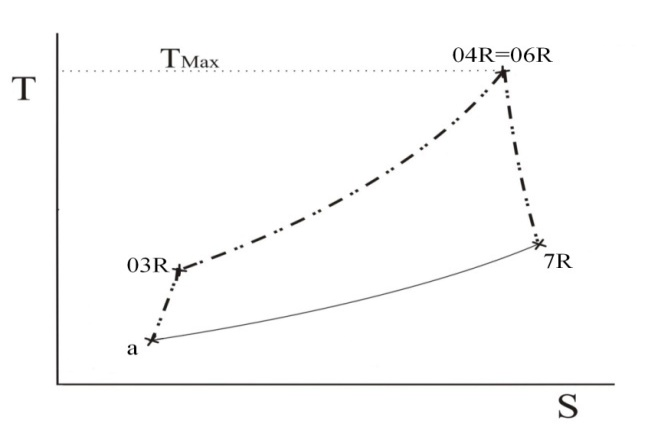
\includegraphics[scale=1]{T-S-Diagram-of-ramjet-engine}\cite{TS}

\section{Introduction}
\section{The Physical Ramjet}
\subsection{Inlet}
\subsection{Combustion Chamber}
\subsection{Nozzle}
\section{The Brayton Cycle}
\subsection{Inlet and Compressor}
\subsection{Combustor}
\subsection{Turbine and Nozzle}
\subsection{Heat Rejection to Atmosphere}
\section{Conclusion}


\bibliography{references}
\bibliographystyle{IEEEtran}
